%%%%%%%%%%%%%%%%%%%%%%%%%%%%%
%Since : Jan/29/2009
%Update: <Mar/13/2013>
% -*- coding: iso-2022-jp -*-
%%%%%%%%%%%%%%%%%%%%%%%%%%%%%

\chapter{ネットワーク基礎演習3}
\section{目的}
sshでwebサーバにアクセスしhtmlファイルを更新しそれを確認することで, リモート操作
に慣れる。簡単なCGI(Common Gateway Interface)スクリプトが動作するかど
うかをパーミッションにより確認することで, UNIX, Linuxにおけるユーザ権限について理
解する。

\section{CGIプログラムを作成する}
これまで実験で作ってきたウェブページは静的で, ウェブページの管理者が内容を更新し
ない限り変化がなかった。また, ウェブページを更新するは, サーバにファイルを送るか,
サーバに直接は入りファイルを更新するしかなかった。このような状況では動的にページ
のデータが更新しなければならないページが作れない。これを解決するためにCGIを用い
る。CGIはサーバ上でプログラムが動き, 様々な処理をする機能である。実験では, 0から
9の数字をプログラムにより表示する。

\paragraph{演習}
\begin{enumerate}
\item ターミナルに, ``ssh cpjweb.center.tsuyama-ct.ac.jp''と入力してEnterキーを押す。
\item 実行すると接続が開始される。相手のコンピュータに初めて接続するときは, 図3の
      ような質問が表示される。``(yes/no)?''というメッセージの後に``yes''と入力してEnter
      キーを押す。
\item パスワードを入力するようメッセージが表示されるので, パスワードを入力する。
\item cdコマンドを用い, ウェブページのデータが保存されているpublic\_htmlに移動する。
\item ``emacs test.cgi''と入力し, プロフラムを書くtest.cgiをemacsで開く。
\item 下記のプログラムソースを入力し保存する。
\item 保存し終えたら, Emacsを終了する。終了するには, Controlとxを同時に押し, 次
      にControlとcを同時に押す。
\item ブラウザで``http://cpjweb.center.tsuyama-ct.ac.jp/\~{}c-○○○/test.cgi''を
      開き, test.cgiが動かないことを確認する。
\end{enumerate}


\begin{figure}[htbp]
\begin{center}
{\small リスト3.1: プログラムソース}
{\small
\begin{verbatim}
#!/usr/bin/perl

print "Content-Type: text/html\n";
print "\n";
for($i = 0; $i < 10; $i++){
  print "$i ";
}
\end{verbatim}
}
\end{center}
\end{figure}

\section{ファイル権限}

先の演習では, 書いたプログラムが動かず想定された結果が表示されなかった。このよう
なことが起こる原因はファイルの権限にある。UNIXでは, ファイルやディレクトリに対し
て, 各ユーザにどのような操作を許可するか, あるいは禁止するかということを設定でき
る。これを権限(permission)と呼ぶ。操作の種類には``読み込み'', ``書き込み'', ``実
行''の3種類がある。ファイルの削除は書き込みの中に含まれる。また, 許可/禁止の対象
となるユーザには``オーナー(所有者)'', ``グループ・ユーザ'', ``その他のユーザ''の
3種類がある。

\subsection{権限の確認}
\paragraph{演習}
\begin{enumerate}
\item コマンドプロンプトに続いて``ls  -l''と入力してEnterキーを押す。
\item 先週の実験とは異なり, 各々のファイルやディレクトリが1行ごと表示されているこ
      とを確認する。
\item 各行の先頭に``- r w - r - - r - -''のような表記があることを確認する。
\end{enumerate}

先ほど確認した``- r w - r - -r- -''のような表記が, それぞれのファイルの権限を示している。
ぞの見方を\figref{fig:permission}に示す。各ユーザの権限は3桁の記号で表される。1桁
目は読み込み(r), 2桁目は書き込み(w),  3桁目は実行(x)を示す。その操作が許可されてい
れば該当するアルファベット(rかwかx)が表示され, 禁止されていれば``-''が表示され
る。``r w - r - -r- -''の例では, オーナーは読み込みと書き込みができ, グループ・ユーザと
その他のユーザは読み込みができる。

\begin{figure}[htbp]
\begin{center}
\fbox{
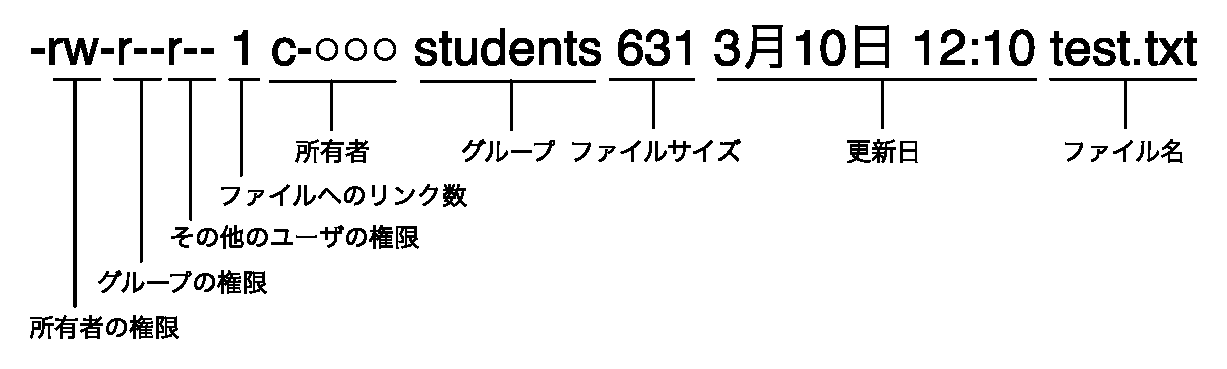
\includegraphics[width=0.8\linewidth]{permission.eps}
}
\caption{権限の説明}
\label{fig:permission}
\end{center}
\end{figure}

\subsection{権限の変更}
ファイルやディレクトリの権限を変更するには``chmod''というコマンドを使用する。
chmodは以下のように使用する。

\vspace{3mm}
  chmod  権限の設定  ファイル名

\vspace{3mm}
権限の設定の仕方はいろいろあるが, ここでは権限を数字で指定するやり方を使う。権限を表
す数字は基本的には3桁の8進数を用いる。もし, r w x r- - r - - (所有者に読み書き実行を許可,
そのほかは読み込みのみ許可)を表す場合は744となる。ここで所有者のみに注目すると,
所有者の権限はrwxとなっている。ここでrを4, wを2, xを1とし, それぞれ有効ならば足
していくとすると, 所有者の権限はrwxなので4+2+1で7となり, 所有者の権限を数字で表
した場合, 7となります。

\paragraph{演習}
\begin{enumerate}
\item cpjwebにsshでアクセスしたままの状態で作業を行う。
\item ホームディレクトリ下のpublic\_htmlにいることを確認する。もしpublic\_htmlにい
      ない場合, cdで移動する。
\item index.htmlの権限を``ls -l''で確認し, 記録する。
\item ``chmod 444 index.html''を実行し, 所有者, グループ, その他のユーザの権限を読み込みのみにする。
\item index.htmlの権限を``ls -l''で読み込みのみになっていることを確認する。
\item emacs index.htmlを実行し, ファイルを開く。
\item 編集しようとすると, read onlyと下の方に表示されるか確認する。
\item ファイルの権限を元にもどす。コマンドは各自考える。
\item index.htmlの権限を``ls -l''で元に戻ったか確認する。
\end{enumerate}

\section{プログラムを動くようにする}
プログラムを動くようにするには実行権限を与えなければならない。特に, CGIの場合所
有者以外(webサーバ)が実行するので所有者以外にもファイルを読み込みと実行の権限を
与えなければならない。つまりファイルの権限をrwxr-xr-xとしなければならない。
動かないtest.cgiの権限をchmodで変更し動くようにする。

\paragraph{演習}
\begin{enumerate}
\item cpjwebにsshでアクセスしたままの状態で作業を行う。
\item ホームディレクトリ下のpublic\_htmlにいることを確認する。もしpublic\_htmlにい
      ない場合, cdで移動する。
\item test.cgiの権限を``ls -l''で確認し記録する。
\item ``chmod''を用い, 権限をrwxr-xr-xにする。
\item test.cgiの権限を``ls -l''で確認する。
\item 予定通りrwxr-xr-xとなっていれば, ブラウザで
      ``http://cpjweb.center.tsuyama-ct.ac.jp/\~{}c-○○○/test.cgi''を開き0から
      9まで表示されるか確認する。
\end{enumerate}

\section{パスワードの変更}
パスワードは初期に設定されたものでは, 誰がどのようなパスワードか分かってしまう。
そこで, 実験室で使うLinux環境用のパスワードの変更を行う。これまで実験で使ってき
たLinux環境用のユーザの情報は第1回で説明したとおりcpjsvという名前のコンピュータ
で管理している。なので, cpjsvのパスワードを変えることで, Linux環境用のパスワード
を変更することができる。ただし, ウェブサーバは管理が別になっているので注意するこ
と。

\paragraph{演習}
\begin{enumerate}
\item sshでcpjsv(cpjsv.center.tsuyama-ct.ac.jp)にアクセスする。
\item ログインに成功したら, ``passwd''と入力してEnterキーを押す。
\item 現在のパスワードを聞いてくるので, 入力する。
\item パスワードがあっていれば, 新しいパスワードを聞いてくるので入力する。
\item 再び新しいパスワードを聞いてくるので, 先ほどと同じパスワードを入力する。
\item パスワードの不一致, 新しいバスワードが単純などの理由でパスワードが変更でき
      ない場合がある。その場合は2からの作業を繰り返し行う。
\item cpjsvからログアウトする。
\end{enumerate}

\section{演習課題}

\begin{enumerate}
\item index.htmlの権限は, はじめどうなっていたか書け。

\item 権限を変更する前のtest.cgiの権限を書け。

\item 権限を変更したtest.cgiはうまく実行できた。なぜ実行できるようになったか, 権
      限という言葉を使って説明せよ。

\item r w - r w - - - -、r w x - - x r - x という権限を表す数字を書け。

\item 755、664で表される権限を答えよ。

\item 権限を644など3桁の数字を用い表した。権限を表す3桁の数字がどのようなルール
      で決まるか説明せよ。(ヒント: rwxの許可不許可を2進数として考えてみるとわかる。)
\end{enumerate}
